% tikzpic.tex
\documentclass[crop,tikz]{standalone}% 'crop' is the default for v1.0, before it was 'preview'
%\usetikzlibrary{...}% tikz package already loaded by 'tikz' option
\usepackage{amsmath,amsthm,amssymb,mathrsfs,amsfonts,dsfont}
\usetikzlibrary{plotmarks}

\begin{document}
    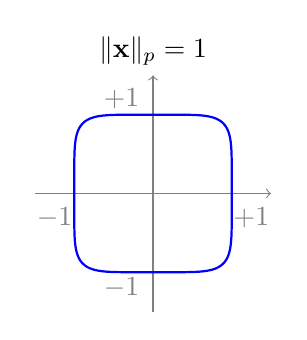
\begin{tikzpicture}[scale=1]
        \draw[->, gray] (-1.5,0) -- (1.5,0);
        \draw[->, gray] (0,-1.5) -- (0,1.5);
        % X ticks
        \draw (-1,0.05) -- (-1,-0.05) node[xshift=-0.25cm, below, gray] {$-1$};
        \draw (1,0.05) -- (1,-0.05) node[xshift=0.25cm, below, gray] {$+1$};
        % Y ticks
        \draw (0.05,-1) -- (-0.05,-1) node[yshift=-0.2cm, left, gray] {$-1$};
        \draw (0.05,1) -- (-0.05,1) node[yshift=0.2cm, left, gray] {$+1$};

        % p-norm
        \draw[domain=0:370,samples=370,smooth,variable=\t,thick,blue]
        plot ({sign(cos(\t)) * abs(cos(\t))^(1/3)}, {sign(sin(\t)) * abs(sin(\t))^(1/3)});
        \node[above,black] at (0.0, 1.5) {$\Vert \mathbf{x} \Vert_p = 1$};
    \end{tikzpicture}
\end{document}